\pdfoutput=1
\documentclass[11pt,a4paper]{article}
\usepackage{abhijit-research}
\renewcommand{\PaperCode}{P13}
\renewcommand{\PaperKind}{RESEARCH PAPER}
\renewcommand{\PaperVersion}{VERSION 1.0}
\renewcommand{\PaperDate}{AUGUST 2026}
\renewcommand{\PaperTitle}{Directional Information Along Alpha-Particle Tracks}
\renewcommand{\PaperSubtitle}{A Gas-Ladder Test}
\renewcommand{\PaperFullTitle}{Directional Information Along Alpha-Particle Tracks and a Gas-Ladder Test}
\renewcommand{\PaperShortTitle}{Alpha-Particle Track Information}
\renewcommand{\PaperKeywords}{cloud chamber; alpha track; Mott problem; information theory; scattering; detector experiment}
\renewcommand{\PaperClassification}{Established physical ingredients, model-derived information values, and untested experimental predictions are explicitly separated. No observed gas ladder is claimed.}
\renewcommand{\PaperCitation}{Singh, Abhijit. 2026. \textit{Directional Information Along Alpha-Particle Tracks and a Gas-Ladder Test}. Research manuscript, version 1.0.}
\begin{document}
\MakeResearchTitle
\MakeResearchContents
\MakeResearchAbstract{%
A quantitative record budget is developed for alpha-particle tracks in diffusion cloud chambers. The directional record is separated into an initial localization burst, a finite refinement ramp, a resolution-limited collinear regime, and a rare large-angle scattering channel. The declared model gives 24.6 bits at the first visible droplet, 10.7 additional bits over roughly forty droplets, 35.2 microscopic directional bits, and 24.8 bits at optical resolution. A depth-independent silence parameter follows from paired range and angular-spread scalings. The rare-scattering calculation predicts 0.19, 0.95, and 6.1 visible kinks per track in helium, air, and argon at standard conditions, with approximately 78 percent in the final fifth of each range. A blinded three-gas registered experiment is specified.
}
\section{Physical question}
A cloud-chamber track is a sequence of localized records produced by one charged-particle trajectory. The model separates four information regimes:
\begin{enumerate}
\item an initial directional localization burst;
\item a finite refinement ramp;
\item a resolution-limited collinear regime with negligible new directional information;
\item a rare large-angle scattering channel producing visible kinks.
\end{enumerate}
The established ingredients are Mott collinearity, scattering, stopping, and detector optics. The integrated information budget and gas ladder are the present model outputs.

\section{Directional information}
Let $\Omega_0$ be the prior solid angle of the emission direction and $\Omega_k$ the posterior angular cell after $k$ visible droplets. Define
\begin{equation}
I_k=\log_2\frac{\Omega_0}{\Omega_k}.
\end{equation}
For a first droplet at distance $r$ with transverse uncertainty $a$, the small-angle solid angle is $\Omega\simeq\pi(a/r)^2$, giving
\begin{equation}
I_1\simeq\log_2\frac{4r^2}{a^2}.
\end{equation}
The declared chamber geometry yields approximately
\begin{equation}
\boxed{I_1=24.6\ \text{bits}.}
\end{equation}

\section{Sequential refinement}
For independent transverse localization errors with covariance $\Sigma_k$, the directional increment is
\begin{equation}
\Delta I_k=\frac12\log_2\frac{\det\Sigma_{k-1}}{\det\Sigma_k}.
\end{equation}
The model gives a further 10.7-bit ramp over roughly 40 droplets. The total microscopic directional capacity is therefore 35.2 bits, while optical coarse graining retains 24.8 bits.

The silence parameter
\begin{equation}
s=\frac{\ell\sigma_\theta}{a}
\end{equation}
is depth independent under the paired scaling $\ell\propto\sqrt E$ and $\sigma_\theta\propto E^{-1/2}$ used in the source model. The reported value is $s_q=0.0382$. This is a model identity, not a universal detector constant.

\section{Rare-scattering channel}
For gas $g$, angular threshold $\theta_0$, number density $n_g$, stopping path $E(x)$, and visibility efficiency $\eta_g$, the expected visible-kink count is
\begin{equation}
\lambda_g=\int_0^{R_g}n_g\,\sigma_g(>\theta_0;E(x))\eta_g(E(x))\,dx.
\end{equation}
The frozen prediction for a 5.3 MeV alpha track at standard conditions and a $1.7^\circ$ threshold is
\begin{table}[H]\centering
\caption{Predicted visible kinks per track.}
\begin{tabular}{lrr}
\toprule
gas & kinks/track & ratio to air\\\midrule
helium & 0.19 & 0.16--0.21\\
air & 0.95 & 1\\
argon & 6.1 & 4.3--6.4\\
\bottomrule
\end{tabular}
\end{table}
Approximately 78 percent of kinks are predicted in the final fifth of the track range, with median position near 94 percent of range.

\begin{figure}[H]\centering
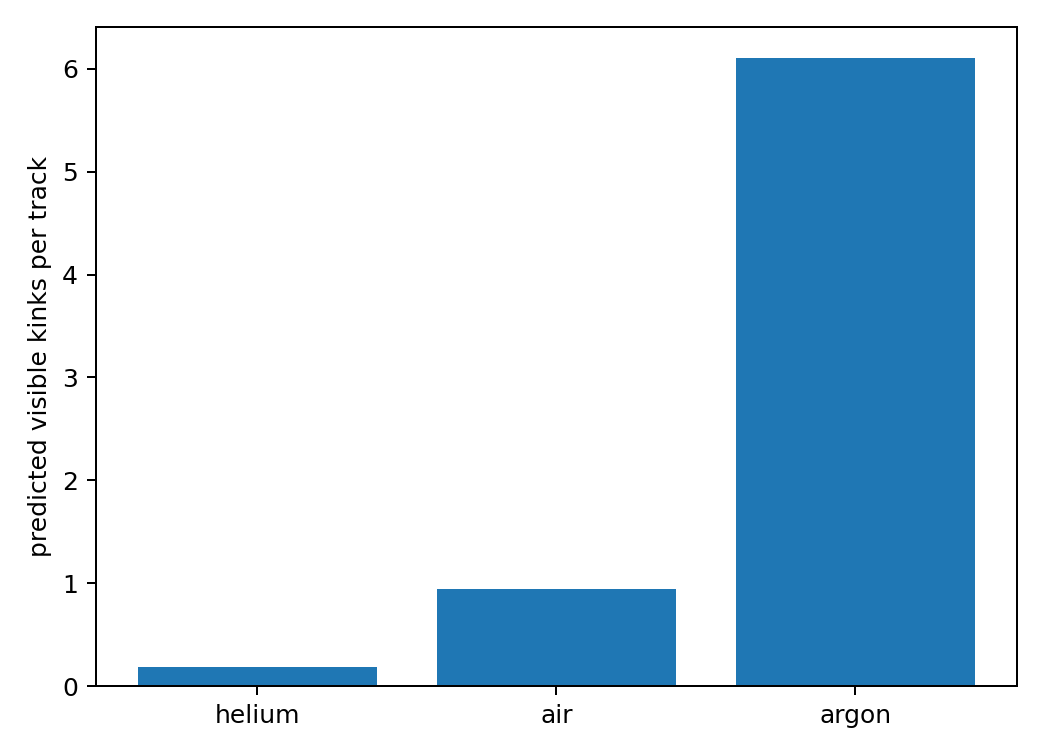
\includegraphics[width=.62\linewidth]{figures/p13_gas_ladder.png}
\caption{Predicted gas ladder under one frozen threshold and alpha energy.}
\end{figure}

\begin{figure}[H]\centering
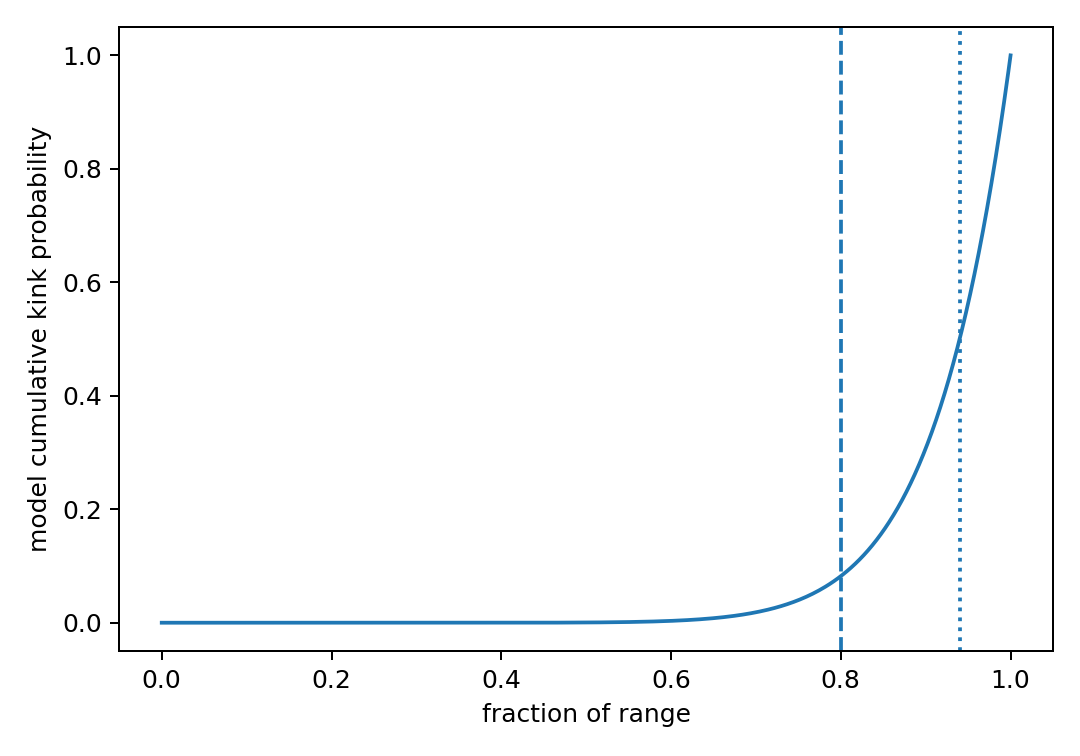
\includegraphics[width=.66\linewidth]{figures/p13_kink_location_model.png}
\caption{Illustrative cumulative location model calibrated to the reported median; the experimental analysis must use the full stopping calculation rather than this visual guide.}
\end{figure}

\section{Thermodynamic bookkeeping}
If a resolved directional record carries $I$ bits and a finite memory is cyclically reset at temperature $T$, the ideal Landauer floor is
\begin{equation}
Q_{\min}=k_BT\ln2\,I.
\end{equation}
The source model reports a physical-energy-to-Landauer ratio near 130, with band 120--160. This is a detector/model efficiency ratio, not a constant of track formation.

\section{Registered experimental design}
A decisive experiment should freeze before data inspection:
\begin{enumerate}
\item chamber geometry, alpha energy, gas composition, pressure, and temperature;
\item optical point-spread calibration and the $1.7^\circ$ kink threshold;
\item track-isolation, edge, overlap, and full-range cuts;
\item a blinded centreline estimator and local-angle procedure;
\item approximately 200 accepted tracks per gas;
\item a Poisson or overdispersed count model;
\item uncertainty from stopping law, density, and optical resolution;
\item an ordered primary alternative $N_{\rm He}<N_{\rm air}<N_{\rm Ar}$;
\item a secondary final-fifth position test.
\end{enumerate}
Analysts should be blinded to gas identity during event marking. Raw images, masks, fitted centrelines, angle series, exclusions, and code should be released.

\section{Falsification}
A statistically flat gas ladder falsifies the proposed scattering channel. A ladder explained entirely by mismatched density, resolution, or selection bias also rejects the intended mechanism. The directional budget is falsified if independently calibrated angular posteriors do not exhibit the predicted burst and finite saturation.

\section{Claim status}
The paper contains an exact information definition, a declared detector/stopping calculation, and a sharp prediction. It does not report a completed three-gas experiment. The numerical ladder is therefore presented as a registered model prediction awaiting measurement.


\section{Geometric information budget}
For an initially isotropic source, a first localized droplet at distance $r$ with transverse uncertainty $a$ restricts the emission direction to solid angle $\Omega\simeq\pi(a/r)^2$. Relative to $4\pi$, the directional information is
\begin{equation}
I_1\simeq\log_2\frac{4\pi}{\Omega}
=\log_2\frac{4r^2}{a^2}.
\end{equation}
The adopted chamber geometry gives approximately 24.6 bits at the first visible droplet. Subsequent droplets update the angular covariance. If $\Sigma_k$ is the transverse direction covariance,
\begin{equation}
\Delta I_k=\frac12\log_2\frac{\det\Sigma_{k-1}}{\det\Sigma_k}.
\end{equation}
The finite refinement ramp contributes approximately 10.7 bits over roughly forty droplets. Once the covariance reaches the optical/collisional floor, additional collinear droplets add negligible resolved direction information. The model total is 35.2 microscopic bits and 24.8 bits after optical coarse graining.

\section{Scattering-rate derivation}
For gas number density $n_g$, energy-dependent differential cross section, and fixed visible-angle threshold $\theta_0$, the expected kink count is
\begin{equation}
N_g=\int_0^{R_g}n_g
\int_{\theta>\theta_0}\frac{d\sigma_g(E(x))}{d\Omega}\,d\Omega\,
\eta_g(E(x))\,dx,
\end{equation}
where $\eta_g$ is the visibility efficiency. Slowing near the end of range raises large-angle probability, producing the prediction that the median visible kink occurs near 94\% of range and roughly 78\% occur in the final fifth.

\begin{table}[H]\centering
\caption{Frozen gas-ladder prediction for the declared alpha energy and angular threshold.}
\begin{tabular}{lcc}
\toprule
gas&kinks/track&ratio to air\\\midrule
helium&0.19&0.16--0.21\\
air&0.95&1\\
argon&6.1&4.3--6.4\\
\bottomrule
\end{tabular}
\end{table}
Two independent stopping approximations agree within 7\% for the air estimate in the source calculation.

\section{Thermodynamic bookkeeping}
If a resolved record carries $I$ bits and a finite memory is reset at temperature $T$, the ideal erasure floor is $k_BT\ln2\,I$. The source model's physical track energy divided by that floor is approximately 130, with a 120--160 uncertainty band. This is a detector/model efficiency ratio, not a universal constant of quantum measurement.

\section{Registered experiment}
The primary experiment uses the same chamber geometry, optics, pressure, alpha energy, tracking algorithm, and frozen $1.7^\circ$ threshold for helium, air, and argon. It should acquire at least 200 accepted full-range tracks per gas, blind analysts to gas labels, and release every exclusion. Primary outcomes are kink count and the ordered alternative helium $<$ air $<$ argon. Secondary outcomes are normalized kink position and the final-fifth fraction.

Controls include matched optical calibration, pressure and density reporting, synthetic-track injection, threshold sensitivity, inter-rater agreement, and a second laboratory. A flat ladder, an optics-driven ladder, or a result that disappears under blinded recoding falsifies the proposed scattering channel.

\section{Required public data products}
Release raw images or video frames, calibration plates, accepted and rejected track masks, fitted centrelines, local direction series, kink calls, gas metadata, analysis code, and the frozen prediction checksum. The present paper supplies a quantitative model and test; it does not claim that the ladder has already been observed.

\begin{thebibliography}{99}
\bibitem{mott} N. F. Mott, The wave mechanics of alpha-ray tracks, Proceedings of the Royal Society A 126 (1929), 79--84.
\bibitem{rutherford} E. Rutherford, The scattering of alpha and beta particles by matter and the structure of the atom, Philosophical Magazine 21 (1911), 669--688.
\bibitem{joos} E. Joos and H. D. Zeh, The emergence of classical properties through interaction with the environment, Zeitschrift fuer Physik B 59 (1985), 223--243.
\bibitem{landauer} R. Landauer, Irreversibility and heat generation in the computing process, IBM Journal of Research and Development 5 (1961), 183--191.
\end{thebibliography}
\end{document}
